We build a Facebook App\footnote{Name and link omitted
for anonymity.} to collect information about users, 
their interactions and preferences.  
%data about Facebook users and their Facebook friends
%are collected through our Facebook App. 
Our dataset contains information about each App user, 
along with a subset of information about their friends visible to the App.
The data collection is performed with full
permission from the user and in accordance with an approved Ethics
Protocol\footnote{Link omitted for anonymity.}.

Over 200 users installed the Facebook App sometime during the
evaluation period. At any time, around 100 users are actively using the
App. From these core App users, the App has access to their 
detailed Facebook profiles with and their interactions with a total of 39,850 friends.
%interaction data.  
While we have complete interaction data for the App
users with their friends, and profile data (including
wall post data) for the App users and friends, we do not have complete
interactions for the App users' friends (unless they themselves are
App users).  Hence in the forthcoming analysis, we limit our
evaluation to App users for which we are assured to have full
interaction data.

Our App tracks many user (and their friends') details and interactions on
Facebook. Interactions that occur through wall posts provided a rich
variety of content and interaction data.  We distinguish four
Facebook items from wall posts: general posts (e.g., status updates,
activity updates such as new friends, and interactions such as the
user liked these pages), links, photos and videos. Four main
interactions on these items are permitted by Facebook: posting an item
to a friend's wall, commenting, liking, and tagging\footnote{Some
Facebook interaction features such as liking comments were introduced
after App user studies began and so are not tracked.}.  The App does not
track deletions of these items and interactions (e.g., unlike) for performance reasons and
we found very few deletions during an initial testing stage.

%% Scott edited up to this point: please don't undo unless something
%% stated is incorrect.  We cannot use the name LinkR b/c it reveals
%% who we are.  I deleted some details of the ethics protocol as they
%% are not needed in this submitted version of the paper for review,
%% can add in camera-ready if needed.  Changed object -> item to be
%% consistent with later terminology.

%% Nguyen: please edit from this point on, only including statistics
%% that are relevant to data shown in the various plots, plus age
%% info as well (since this is useful to know).  So for example, 
%% you can comment out all non-gender, non-age demographics (locale, 
%% location, etc.) as well as unused table data (e.g., note that *only*
%% education and school -- first two rows of Table 3 are needed).
%% SVN has the record if we ever need to add this data back in.
%%
%% I did a search replace of LinkR with App... need to fix some 
%% awkward mentions.
%%
%% In short make sure all data mentioned is relevant to evaluation
%% section, other information is superfluous.

We summarize relevant basic statistics of the data in Table~\ref{tab:interactions}-\ref{tab:interests} below.
The tables distinguish the data from the App users and from
all App users and friends. Table~\ref{tab:interactions}
summarises the number of records for each item (row) and interaction (column)
combination. Table~\ref{tab:demographics} shows 
some demographics from user profiles\footnote{Note that
count of schools are not unique as each user can attend more than one
degree of the same type.}. Figure~\ref{fig:agegroups} shows the age distribution in our dataset\footnote{Many users did not specify a birthday or birth year, and a number of 100+ year old users are not shown.}. Table~\ref{tab:history} shows user profile data that are related to education and work information. 
%%lexing: shouldn't tab:history be just merged into demographics?? i'm leaving it as is for now
The final
set of data collected is about group memberships and interests, in Table~\ref{tab:interests}.
This set of data provides the
implicit groups of interests expressed by users (e.g. movies,
music, television) and the explicit actions of users to join groups (e.g. groups
with membership restrictions and pages, which essentially are groups
without membership restrictions).

We collect numerous interaction and groups data for determining common preferences on Facebook. Some of these online interactions suggest real-world interactions as seen in photos and videos with tagging. Tagging of friends in photos and videos have some drawbacks, but we assume that tags are correct and correspond to real people interacting in real environments. The virtual interactions and virtual groups provide insight into Facebook communities and their diversity of topics, users and interactions with non-friends.


% 18th Jan 2012
\begin{table}
\centering
\begin{tabular}{|>{\small}l|>{\small}r|>{\small}r|>{\small}r|>{\small}r|}
\hline
\textbf{App Users} & \textbf{Posts} & \textbf{Tags} & \textbf{Comments} & \textbf{Likes} \\
\hline
\textbf{Wall} & 27,955 & 5,256 & 15,121 & 11,033 \\
\hline
\textbf{Link} & 3,974 & --- & 5,757 & 4,279 \\
\hline
\textbf{Photo} & 4,147 & 22,633 & 8,677 & 5,938 \\
\hline
\textbf{Video} & 211 & 2,105 & 1,687 & 710 \\
\hline
\hline
\textbf{App Users} & \textbf{Posts} & \textbf{Tags} & \textbf{Comments} & \textbf{Likes} \\
\textbf{and Friends} & & & & \\
\hline
\textbf{Wall} & 3,384,740 & 912,687 & 2,152,321 & 1,555,225 \\
\hline
\textbf{Link} & 514,475 & --- & 693,930 & 666,631 \\
\hline
\textbf{Photo} & 1,098,679 & 8,407,822 & 2,978,635 & 1,960,138 \\
\hline
\textbf{Video} & 56,241 & 858,054 & 463,401 & 308,763 \\
\hline
\end{tabular}
\caption{Number of records in Items and Interactions Tables. Rows are type of Facebook item and columns are type of Facebook interaction.}
\label{tab:interactions}
\end{table}




% 18th Jan 2012
\begin{table}
\centering
\begin{tabular}{|>{\small}p{2cm}|>{\small}r|>{\small}r|}
\hline
\textbf{Table} & \textbf{\#Records} & \textbf{\#Records} \\
& \textbf{(App Users)} & \textbf{(App User} \\
& & \textbf{and Friends)} \\
\hline
Users & 103 & 39,850 \\
\hline
\hline
\textbf{Column} & \textbf{\#Non-empty} & \textbf{\#Non-empty} \\
& \textbf{(App Users)} & \textbf{(App User} \\
& & \textbf{and Friends)} \\
\hline
Gender & 102 & 36,401 \\
%\hline
%Locale & 103 & 36,900 \\
%\hline
%Timezone & 103 & 117 \\
\hline
Birthday & 103 & 27,624 \\
%\hline
%Hometown\par Location & 63 & 17,584 \\
%\hline
%Current\par Location & 71 & 20,088 \\
\hline
\hline
\textbf{Breakdown} & \textbf{Count} & \textbf{Count} \\
& \textbf{(App Users)} & \textbf{(App User} \\
& & \textbf{and Friends)} \\
\hline
Male & 73 & 19,742 \\
\hline
Female & 29 & 16,659 \\
\hline
High School & 104 & 29,503 \\
\hline
College & 115 & 29,223 \\
\hline
Graduate School & 56 & 7733 \\
\hline
%%lexing: isn't it just "College" and not "Degree:College"
%Degree:\par High School & 104 & 29,503 \\
%\hline
%Degree:\par College & 115 & 29,223 \\
%\hline
%Degree:\par Graduate School & 56 & 7733 \\
%\hline
\end{tabular}
\caption{App user demographics.}
\label{tab:demographics}
\end{table}


\begin{figure}[t!]
\centering
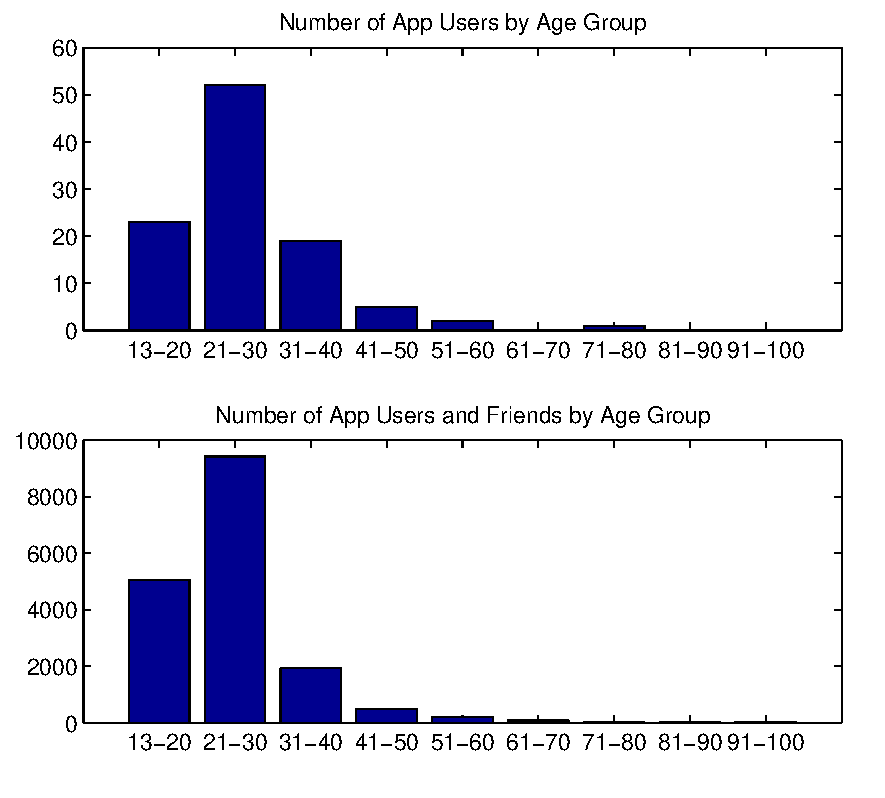
\includegraphics[scale=0.55]{data/age_groups_all.pdf}
\vspace{-10pt}
\caption{Number of App Users by Age Groups.}
\label{fig:agegroups}
\end{figure}


\begin{comment}
\hline
Age: 11-15 & 0 & 208 \\
\hline
Age: 16-20 & 23 & 4,850 \\
\hline
Age: 21-25 & 28 & 6,257 \\
\hline
Age: 26-30 & 24 & 3,162 \\
\hline
Age: 31-35 & 10 & 1,377 \\
\hline
Age: 36-40 & 9 & 588 \\
\hline
Age: 41-45 & 4 & 293 \\
\hline
Age: 46-50 & 1 & 200 \\
\hline
Age: 51-55 & 2 & 116 \\
\hline
Age: 56-60 & 0 & 90 \\
\hline
Age: 61-65 & 0 & 60 \\
\hline
Age: 66-70 & 0 & 25 \\
\hline
Age: 71-75 & 1 & 15 \\
\hline
Age: 76-80 & 0 & 4 \\
\hline
Age: 81-85 & 0 & 11 \\
\hline
Age: 86-90 & 0 & 6 \\
\hline
Age: 91-95 & 0 & 16 \\
\hline
Age: 96-100 & 0 & 20 \\
\hline
Age: 100+ & 1 & 55 \\
\end{comment}



% 18th Jan 2012
\begin{table}
\centering
\begin{tabular}{|>{\small}p{2cm}|>{\small}r|>{\small}r|}
\hline
\textbf{Table} & \textbf{\#Records} & \textbf{\#Records} \\
& \textbf{(App Users)} & \textbf{(App User} \\
& & \textbf{and Friends)} \\
\hline
Education & 275 & 66,462 \\
%\hline
%School & 275 & 27,635 \\
%\hline
%School Classes & 89 & 5,825 \\
%\hline
%School Class & 115 & 8,313 \\
%With Friends & & \\
%\hline
%School Degree & 275 & 1,730 \\
%\hline
%School Degree & 96 & 14,429 \\
%Concentration & & \\
%\hline
%School & 80 & 12,575 \\
%With Friends & & \\
\hline
Work & 134 & 28,610 \\
%\hline
%Work Employer & 134 & 19,053 \\
%\hline
%Work Position & 134 & 7,947 \\
%\hline
%Work Projects & 9 & 1,336 \\
%\hline
%Work Projects & 0 & 4,466 \\
%With Friends & & \\
%\hline
%Work & 21 & 5,204 \\
%With Friends & & \\
\hline
\end{tabular}
\caption{User history.}
\label{tab:history}
\end{table}


% 18th Jan 2012
\begin{table}
\centering
\begin{tabular}{|>{\small}p{2cm}|>{\small}r|>{\small}r|}
\hline
\textbf{Table} & \textbf{\#Records} & \textbf{\#Records} \\
& \textbf{(App Users)} & \textbf{(App User} \\
& & \textbf{and Friends)} \\
%\hline
%Activities & 394 & 92,148 \\
%\hline
%Books & 266 & 52,690 \\
%\hline
%Favorite Athletes & 58 & 23,009 \\
%\hline
%Favorite Teams & 35 & 14,772 \\
\hline
Groups & 3,792 & 778,751 \\
%\hline
%Inspirational People & 39 & 7,815 \\
%\hline
%Interests & 153 & 36,085 \\
\hline
Movies & 616 & 149,197 \\
\hline
Music & 1,245 & 318,296 \\
\hline
Page Likes & 11,973 & 3,004,360 \\
%\hline
%Sports & 48 & 8,663 \\
\hline
Television & 819 & 144,308 \\
\hline
\end{tabular}
\caption{Groups of Interests Tables}
\label{tab:interests}
\end{table}





\begin{comment}
% 18th Jan 2012
\begin{table}
\centering
\caption{\small All other records.}
\label{tab:all}
\begin{tabular}{|>{\small}p{2cm}|>{\small}r|>{\small}r|}
\hline
\textbf{Table} & \textbf{\#Records} & \textbf{\#Records} \\
& \textbf{(App Users)} & \textbf{(App User} \\
& & \textbf{and Friends)} \\
\hline
Activities & 394 & 92,148 \\
\hline
Books & 266 & 52,690 \\
\hline
Education & 275 & 66,462 \\
\hline
Favorite Athletes & 58 & 23,009 \\
\hline
Favorite Teams & 35 & 14,772 \\
\hline
Friends & 35,869 & 39,873 \\
\hline
Groups & 3,792 & 778,751 \\
\hline
Inspirational People & 39 & 7,815 \\
\hline
Interests & 153 & 36,085 \\
\hline
Location & 206 & 6,636 \\
\hline
Movies & 616 & 149,197 \\
\hline
Music & 1,245 & 318,296 \\
\hline
Pages & 11,973 & 3,004,360 \\
\hline
School & 275 & 27,635 \\
\hline
School Classes & 89 & 5,825 \\
\hline
School Class With Friends & 115 & 8,313 \\
\hline
School Degree & 275 & 1,730 \\
\hline
School Degree Concentration & 96 & 14,429 \\
\hline
School With Friends & 80 & 12,575 \\
\hline
Sports & 48 & 8,663 \\
\hline
Sports With Friends & 26 & 3,577 \\
\hline
Television & 819 & 144,308 \\
\hline
Users & 103 & 36,900 \\
\hline
Work & 134 & 28,610 \\
\hline
Work Employer & 134 & 19,053 \\
\hline
Work Position & 134 & 7,947 \\
\hline
Work Projects & 9 & 1,336 \\
\hline
Work Projects With Friends & 0 & 4,466 \\
\hline
Work With Friends & 21 & 5,204 \\
\hline
\end{tabular}
\end{table}
\end{comment}

